\chapter{The blood filter}
	
There is no life without metabolizing, and metabolism always produces variety of waste products, which accumulated in the tissues are toxic to the organism. Some of them are removed from the body by respiratory trucks, others through digestive system and some of them are extracted through the sweat gland. However, there is no doubt that the urinary system plays the major role in waste extraction.

The main organs of the urinary system are the kidneys. It is them, who perform the filtering function. The remaining ones,  ureters, urinary bladder, and urethra, form the urinary tracks and are responsible only for transforming and storing the urine. In this chapter the anatomy and physiology of the kidneys will be briefly introduced.

\section{Structure of the kidney} 

The kidneys are  bean-shaped, usually paired structures located at the back of the abdominal cavity in the retroperitoneal space. They lie on at the level of vertebrae T12 to L3.
The right kidney is slightly lower than the left one, because of the presence of the liver \cite{saladin, health_and_disease}. 

The average healthy adult kidney weights around 150\,g, is 11\,cm long, 6\,cm wide and 3\,cm thick \cite{kidney_dimensions, saladin}. As mentioned before, humans usually have two kidneys, however not always.  Some people are born with only one of them.  In such case, the present kidney is as heavy and big as the two kidneys together would be. In most cases it doesn't affect normal live. 

The kidneys are surrounded and protected by three types of connective tissue, from the outter part: 
\begin{inparaenum}[(1\upshape)]
\item \textit{renal fascia} anchoring the kidneys and the neighbouring organs to the abdominal wall
\item \textit{adipose capsule}, which is a layer of fat holding the kidney in a place
\item \textit{renal capsule}, made of fibrous tissue firmly enclosing the organ and protecting it from traumas and infections \cite{saladin, health_and_disease}.
\end{inparaenum} In the medial concave surface, there is a~slit called \textit{hillum}, which is the place where the  renal  artery enters and the renal vein and the ureter leave the kidney. The hillum extens into the \textit{renal sinus}, which is a large cavity occupied by blood and lymphatic vessels, nerves, urine-collecting structures and adipose tissue \cite{health_and_disease}.

The renal parenchyma is divided into two major parts: 
\begin{inparaenum}[(1\upshape)]
\item the outer 1\,cm thick portion of the kidney,  \textit{renal cortex}
\item the inner \textit{renal medulla}
 \cite{saladin, health_and_disease}.
\end{inparaenum}
The cortex projects into the kidney forming \textit{renal columns}, which divide the medulla into 10-14 \textit{renal pyramids}. Each of them has a characteristic shape of cone with wide base facing the cortex and the tip attached to the sinus called \textit{renal papilla}.  The papilla of the each pyramid points towards the \textit{minor calyx} collecting its urine. Few of them converge into the \textit{major calyx}, whereas the all latter ones form the funnel-shaped basin,  \textit{the renal pelvis}, which is the extension of the \textit{ureter} transforming the urine to the bladder \cite{saladin, health_and_disease, mosby}. The gross anatomy of the kidney is illustrated on the Figure \ref{fig:kidney_anatomy}.

	%\vspace*{-1.5cm}
\begin{figure}[H]
		\centering
		\includegraphics [height = 8cm]{kidney2}
		\caption [Gross kidney anatomy]{The structure of the kidney \cite{saladin}}
		\label{fig:kidney_anatomy}
	\end{figure}
\subsection{The nephron} 

As it is with most of the aspects of the human anatomy, the most interesting features of the kidney are invisible with naked-eye. 
The basic microscopic functional units of the kidney are nephrones. Above million of them enables the kidney to perform its functions \cite{health_and_disease}. Each of them is a tiny coiled tube, the \textit{renal tubule}, with a bulb at the end, the \textit{renal corpuscle}, and extends through both the cortex and the medulla. 

The renal corpuscle is composed of the two-layered \textit{glomerular (Bowman) capsule} enclosing the
\textit{glomelurus}, which is a cluster of capillaries. The renal tubule is a~duct leading from the glomelural capsule to the pyramid papilla. It can be divided into several regions, subsequently from the glomerular corpuscle: 
\begin{inparaenum}[(1\upshape)]
\item The \textit{proximal convoluted tubule} (PCT)
\item the \textit{nephron loop (loop of Henle)}, which consists of the \textit{descending and ascending limbs}
\item The \textit{distal convoluted tubule }(DCT)
\item the \textit{collecting duct} receiving the fluids from the DCTs of few nephrons. Multiple of them merge and form papillary ducts, which lead  to the minor calyx.
% \cite{saladin, health_and_disease}.
\end{inparaenum}
Each of the segment has individual cellular appearance and function.

Every functional unit of the kidney is supplied with the blood by the small blood vessel called \textit{the proximal convoluted tubule} whereas the \textit{efferent  arteriole} takes it back. The blood leaving the nephron, flows  into  a
network of \textit{peritubular  capillaries} surrounding the renal tubule. The particular parts of the nephron are depicted on the Figure \ref{fig:nephron}.

\begin{figure}
		\centering
		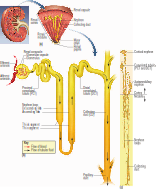
\includegraphics [width = \textwidth]{nephron}
		\caption [nephron]{The structure of the kidney \cite{saladin}}
		\label{fig:nephron}
	\end{figure}



\section{Functions of the kidney} 

Despite of the fact that the key function of the kidneys is purifying the blood, the other ones are equally important. Kidneys are responsible for maintaining homeostasis of all body due to which, all organs can work in optimal environment.
It is crucial for proper functioning of whole organism \cite{mosby}. One can conclude that the role of kidneys is enormously important. The kidneys are involved in the following processes:
\begin{description}
		%\renewcommand\labelitemi{$\blacksquare$}
		\item [Blood filtering.] The kidneys filter the blood from metabolic waste, excess salt and toxins and then excrete unwanted substances in the urine \cite{saladin, health_and_disease, mosby}.
		
		\item [Osmoregulation.]	For proper functioning of the organism, the concentration of the salts in the body has to remain relatively the same. The kidneys, influence this concentration which by controlling the amount of water and solutes excrected from the organism \cite{sturkie1986kidneys}.	
		
		\item [Maintainance of water balance.] The kidneys controll the amount of water conserved and eliminated in the urine so that the amount of body water remains on the stable level \cite{jequier2010water}.
					
		\item [Blood pressure regulation.] Maintaining appropriate blood pressure is achieved in 2 ways: \begin{inparaenum}[(1\upshape)]\item if the blood pressure drops, the kidneys release the enzyme \textit{renin}, which activates a blood protein \textit{angiotensin} making the blood vessels to constrict. What is more, angiotensin triggers the mechanism which increases the absorption of water and sodium increasing blood volume  \item regulating the amount of water, which was mentioned before \cite{guyton1972arterial}. \end{inparaenum} 
			
		\item [Maintainance of the acid-base balance.] The food conteained in our diet can acidify or neutralize the organism. If the pH is outside the tolereable boundaries, enzymes and proteins break down, which in extreme cases can lead to death. Kidneys in collaboration with the lungs are responsible for maintaining healthy pH of the body fluids. While the lungs' task is to regulate carbon dioxide ($CO_{2}$) concentration, the kidney acts by reabsorbing or regenerating bicarbonate ($HCO_{3}^{-}$) from urine and excreting hydrogen ions and fixed acids into it \cite{hamm2015acid}.
	
	\item [Red blood cell production.] If the level of oxygen in the tissue is insufficient, the kidneys release \textit{erythroprotein}, the hormon stimulating the bone narrow to red blood cells production \cite{donnelly2001erythropoietin}. 

\item [Keeping the bones strong.] The kidneys, together with the liver, synthesize the active form of vitamin D called \textit{calcitriol} (1,25-dihydroxycholecalciferol) enabling the body to absorb calcium and phosphorus, crucial minerals for strengthening the bones \cite{williams2009vitamin}.

\item [Prevent the hunger.] In the situation of extreme starvation, the kidneys can synthesize glucose from non-carbohydrate carbon substrates breakind down the other molecules. This phenomena is known as \textit{gluconeogenesis} \cite{newsholme1967control}.

\item [Hormones degradation.] The kidneys takes part in degradation of hormones such as \textit{parathyroid hormone} or \textit{insulin} \cite{emmanouel1980role}. 
%					
	\end{description} 

\subsection{Urine formation} 
Everyday, our kidney filter as much as 200 litres of fluid and excrete 1.5 litres of urine. The process of the urine formation can be divided into 3 stages:
\begin{enumerate}
\item{\textbf{Glomerular filtration}} When the blood enters the glomerulus through the afferent arteriole, the first step begins.  
\item{\textbf{Tubular reabsorption}}
\item{\textbf{Tubular secretion}}
\end{enumerate}


\subsection{glomerular filtration rate}

\section{Kidney diseases} 

 